\documentclass[12pt,a4paper,oneside,DIV=calc]{scrartcl}
\usepackage{polyglossia}
\setdefaultlanguage[variant=british]{english}
\usepackage{url}
\usepackage{amsmath}
\usepackage{amsfonts}
\usepackage{amssymb}
\usepackage{graphicx}
\usepackage{multicol}
\usepackage{multido}
\usepackage{enumitem}
%\usepackage{pdfpages}
\usepackage{nomencl}
\usepackage{subcaption}

%%% Formatting
\usepackage{geometry}
\usepackage{lscape}
\usepackage{longtable}
\usepackage{array}
\newcolumntype{L}[1]{>{\raggedright\let\newline\\\arraybackslash\hspace{0pt}}m{#1}}
\newcolumntype{C}[1]{>{\centering\let\newline\\\arraybackslash\hspace{0pt}}m{#1}}
\newcolumntype{R}[1]{>{\raggedleft\let\newline\\\arraybackslash\hspace{0pt}}m{#1}}
\usepackage{fancyhdr}
\pagestyle{fancy}
\usepackage{marginnote}
\renewcommand*{\marginfont}{\footnotesize \itshape}
\usepackage{setspace}
\setstretch{1.15}
%\setlength{\parindent}{1em}
\usepackage{lastpage}

%%% Colors
\usepackage{xcolor}
\PassOptionsToPackage{dvipsnames}{xcolor}
\definecolor{linkgray}{gray}{0.2}
\definecolor{mygreen}{cmyk}{0.98, 0.00, 0.93, 0.61}

\usepackage[
    backend=biber,
    style=alphabetic,
    citestyle=alphabetic,
    natbib=true,
    url=true, 
    doi=true,
    eprint=false,
    maxbibnames=10
]{biblatex}
\addbibresource{./BDLP.bib}
\renewcommand*{\multicitedelim}{\addcomma\space}

\setcounter{abbrvpenalty}{0}
\setcounter{highnamepenalty}{0}
\setcounter{lownamepenalty}{0}
% If you want to break on URL numbers
\setcounter{biburlnumpenalty}{9000}
% If you want to break on URL lower case letters
\setcounter{biburllcpenalty}{9000}
% If you want to break on URL UPPER CASE letters
\setcounter{biburlucpenalty}{9000}

\usepackage{microtype}

%%% TODO Notes
%\setlength{\marginparwidth }{2.5cm}
\usepackage{xargs} 
\usepackage[colorinlistoftodos,prependcaption,textsize=tiny]{todonotes}
\newcounter{todocounter}  
\newcommandx{\todoc}[2][1=]{\stepcounter{todocounter}\todo[linecolor=yellow,backgroundcolor=yellow!25,bordercolor=yellow,#1]{\sffamily \thetodocounter: #2}}
\newcommandx{\unsure}[2][1=]{\stepcounter{todocounter}\todo[linecolor=blue,backgroundcolor=blue!25,bordercolor=blue,#1]{\sffamily \thetodocounter: #2}}
\newcommandx{\change}[2][1=]{\stepcounter{todocounter}\todo[linecolor=red,backgroundcolor=red!25,bordercolor=red,#1]{\sffamily \thetodocounter: #2}}
\newcommandx{\info}[2][1=]{\stepcounter{todocounter}\todo[linecolor=OliveGreen,backgroundcolor=OliveGreen!25,bordercolor=OliveGreen,#1]{\sffamily \thetodocounter: #2}}
\newcommandx{\improvement}[2][1=]{\stepcounter{todocounter}\todo[linecolor=Plum,backgroundcolor=Plum!25,bordercolor=Plum,#1]{\sffamily \thetodocounter: #2}}

%%%Fonts
\usepackage[utf8]{inputenc}
\usepackage[autostyle]{csquotes}
\usepackage{fontspec}
\defaultfontfeatures{Mapping=tex-text}
\usepackage{xunicode}
\usepackage{xltxtra}
%\setmainfont[Path=fonts/,
%ItalicFont=EBGaramond12-Italic.otf,
%SmallCapsFont=EBGaramondSC12-Regular.otf]{EBGaramond12-Regular.otf}
%\setmainfont[Path=fonts/,
%ItalicFont=OFLGoudyStM-Italic.otf]{OFLGoudyStM.otf}
%\setmainfont[Path=fonts/,
%ItalicFont=Fanwood-Text-Italic.otf]{Fanwood-Text.otf}
%\setmainfont[Path=fonts/,
%ItalicFont=OFLGoudyStM-Italic.otf]{GoudyBookletter1911.otf}
%\setmainfont[Path=fonts/]{Minion-Pro-Display.otf}
%\setmainfont[Path=fonts/,
%ItalicFont=texgyrepagella-italic.otf]{texgyrepagella-regular.otf}
\setmainfont[Path=fonts/,Numbers={OldStyle},
ItalicFont=ArnoPro-Italic.otf]{ArnoPro-Regular.otf}

%\setsansfont[Ligatures=NoCommon, Path=fonts/,
%BoldFont=Din Pro Bold 700.otf,
%ItalicFont=Din Pro Italic 400.otf]{DIN Pro 400.otf}
%\setsansfont[Path=fonts/,
%BoldFont=Raleway-Bold.otf,
%ItalicFont=Raleway-MediumItalic.otf]{Raleway-Medium.otf}
\setsansfont[Path=fonts/,
BoldFont=Raleway-Medium.otf,
ItalicFont=Raleway-LightItalic.otf]{Raleway-Light.otf}
%\setsansfont[Ligatures=NoCommon, Path=fonts/,
%BoldFont=Junction-bold.otf]{Junction-regular.otf}
\newfontfamily\ethbfont[Ligatures=NoCommon, Path=fonts/]{DIN Pro Bold 700.otf}
\newfontfamily\ethbitfont[Ligatures=NoCommon, Path=fonts/]{DIN Pro Black Italic 900.otf}
\newfontfamily\ethitfont[Ligatures=NoCommon, Path=fonts/]{DIN Pro Italic 400.otf}
\newfontfamily\ethfont[Ligatures=NoCommon, Path=fonts/]{DIN Pro 400.otf}

%%% Set Variables
\newcommand{\docAuthor}{Andreas Felderer}
\newcommand{\docMatNr}{19-907-781}
\newcommand{\docTitle}{Big Tech, Merchants of Doubt?}
\newcommand{\docSubTitle}{Facebook and Social Network Addiction\\ A Case Study}
\newcommand{\docTypeofWork}{Case study in ...}
\newcommand{\docLectureTitle}{Big Data, Law, and Policy}
\newcommand{\docLectureNumber}{851-0740-00L}
\newcommand{\docTeacher}{Prof. Stefan Bechtold}
\newcommand{\docUni}{ETH Zürich}
% Semester
\newcommand{\docTerm}{Spring Term 21}
\newcommand{\docTermShort}{ST 21}
\author{\docAuthor}
\title{\docTitle}

%%% Header
%\lhead[]{\small{
\includegraphics[height=8pt]{figures/ETHZ_logo_black.png}{\ethfont{\textit{, \docTermShort}}}} }
\lhead[]{\sffamily\footnotesize{\docUni, {\scriptsize ST} 21}} 
\chead[]{\sffamily\footnotesize{\textit{\docLectureTitle} }}
\rhead[]{\sffamily\footnotesize{\docTeacher}}
%%% Footer
\lfoot[]{\footnotesize{\sffamily\docAuthor; \docMatNr}}%; M.Sc. Science, Technology and Policy} }% 
\cfoot[]{\footnotesize{}}
\rfoot[]{\footnotesize{\sffamily \docTitle \,$\cdot$\,\thepage}}
\usepackage{titlesec}
\titleformat{\section}{\sffamily\Large\bfseries}{\thesection}{1em}{}
\titleformat{\subsection}{\sffamily\large\bfseries}{\thesubsection}{1em}{}
\titleformat{\subsubsection}{\sffamily\large}{\thesubsubsection}{1em}{}
\titleformat{\paragraph}[runin]{\sffamily\normalsize}{\theparagraph}{1em}{}
\titleformat{\subparagraph}[runin]{\normalfont\normalsize\itshape}{\thesubparagraph}{1em}{}

\usepackage{footmisc}
\usepackage[
  	indexonlyfirst,% only index first use%
    xindy,% xindy zum Indexieren verwenden
    nogroupskip,
    acronym,% Separates Akronym-Verzeichnis
    nopostdot,% Kein Punkt am Ende einer Beschreibung im Glossar
    nomain]{glossaries}
%\usepackage{glossary-mcols}
\newacronym{eth}{ETH}{Eidgenössische Technische Hochschule}
\newacronym{fb}{FB}{Facebook}
\newacronym{sns}{SNS}{Social Network Service}
\newacronym{pr}{PR}{Pubblic Relations}

%\nomenclature{ETH}{Eidgenössische Technische Hochschule}
%\nomenclature{
%\nomenclature{SNS}{Social Network Service}
%\nomenclature{PR}{Pubblic Realtions}

\usepackage{xurl}
\usepackage[colorlinks,breaklinks,hyperfootnotes=false]{hyperref}
\hypersetup{urlcolor=mygreen,linkcolor=linkgray,citecolor=mygreen}

%%%%%%%%%%%%%%%%%

%%% Document %%%%

%%%%%%%%%%%%%%%%%
\begin{document}

\def\&{\XeTeXglyph307 }
%%% Titleage
\begin{titlepage}
	\centering
    \vspace*{0.4 cm}
    
\includegraphics[scale = 0.15]{figures/ETHZ_logo_black.png}\\[1.0 cm]	% University Logo
    \textsc{\LARGE Eidgenössische Technische Hochschule Zürich}\\[2.0 cm]
	
	\textsc{\Large \docLectureNumber}\\[0.5 cm]	% Course Code
	%\textsc{\Large \docTypeofWork}\\[0.5 cm] 
	\textsc{\Large \bfseries\sffamily \docLectureTitle}\\[0.5 cm]	% Course Name
	{\large \docTeacher}\\[0.5cm]
	\textsc{\large \docTerm }\\[0.5 cm]
	\rule{\linewidth}{0.2 mm} \\[0.6 cm]

	% Title
	{\huge\bfseries\sffamily \docTitle}\\[0.5 cm]
	% Subtitle
	{\Large\sffamily \docSubTitle}\\
	\rule{\linewidth}{0.2 mm} \\[0.4 cm]
	
	{\Large\itshape \docAuthor \par}
	Matr. Nr. \docMatNr \par
	\href{mailto:afelderer@ethz.ch}{afelderer@ethz.ch} \\[2 cm]

	
	Ich, Andreas Felderer, versichere hiermit, dass ich die von mir eingereichte Arbeit selbstständig verfasst und keine
anderen als die angegebenen Quellen und Hilfsmittel benutzt habe.
\change{Change Language}

	\vfill

% Bottom of the page

	{\large \today \par}
\end{titlepage}
\pagenumbering{Roman}
\thispagestyle{empty}
\begin{center}
    \large\sffamily{\textbf{Abstract}}
\end{center}
\begin{abstract}
In this Case study I explore the science around social network service addiction and the stance of Facebook. 
\end{abstract}
\newpage
\tableofcontents
\newpage

%%% Start of Content
\pagenumbering{arabic} 
\setcounter{page}{3}

%%% Intro
\section{Introduction}
\label{sec:intro}
%\addcontentsline{toc}{section}{Introduction}

\subsection{Motivation}
Over the past decades various industries have fought scientific results, scientists, or even science in general, if the scientific results were putting their profits at risk. 
Some prime examples -- outlined among others in \citet{oreskes_merchants_2010} and \citet{cuveillier_forschung_2020} -- are: 
Big Tobacco (i.e., the world's largest tobacco companies) contesting the link between (second-hand) smoking and cancer for decades, 
Big Oil (i.e., the largest oil companies) contesting the existence of anthropogenic (man made) climate change, 
or the agrochemical industry diverting attention away from pesticides (esp. neonicotinoids\footnote{Neonicotinoids are chemicals used to protect plants from herbivore (plant eating) insects. The seeds of these plants are coated with neonicotinoids which later migrate into all parts of the plant, which is why they are also called \textit{systemic} insecticides. Since these chemicals migrate into all parts of the plant, they also end up in the pollen and reach bees this way, where they cause among others reduced foraging and reproduction \citep{whitehorn_neonicotinoid_2012}.}) towards other causes, in the issue of colony collapse disorder (i.e., bee death).

These reports of industries -- ruled by few large players -- that actively fought scientific evidence over the last couple of decades, raises the question:
\begin{quote}
\itshape
Does Big Tech engage in similar activities?
\end{quote}

As pointed out in \citep{abdalla_grey_2021}, defining Big Tech is not trivial.
For the scope of this paper, however, a precise definition will not be necessary.
The \textquote{Big Five} digital technology firms namely: Alphabet (the parent company of Google), Amazon, Apple, Facebook, and Microsoft can serve as a mental starting point, while remembering that there are many other large and powerful technology companies\footnote{\citet[p 2]{abdalla_grey_2021} define Big Tech as: \textquote{Google, Amazon, Facebook, Microsoft, Apple, Nvidia, Intel, IBM, Huawei, Samsung, Uber, Alibaba, Element AI, OpenAI}.\label{foot:big_tech}}.

Why start with the Big Five? They, have recently\footnote{As of \today.}been ranked in positions 1, 2, 4, 5, and 6 in terms of worldwide market capitalisation (i.e., the number of shares times the current market price).
The only firm surpassing some of the Big Five companies in this ranking, is Saudi Amarco the Saudi Arabian oil company \citep{noauthor_largest_2021}. 
Furthermore, all five companies together amount to a market capitalisation of about \$9.13 \gls{tn} which is about 41\% of the current US gross domestic product, which -- in the first Quarter of 2021 -- was estimated to amount to \$22.06 \gls{tn} \citep{bea_gross_2021}.

Not only are these companies large and powerful, they also predominantly shape the development of large parts of human facing digital technology. 
That is, they control -- in large part -- the design of technologies most humans are using on a daily basis. 
In 2020 more than 80\% of the US population -- 18 years and older -- owned a smartphone and used it at least once per month, 46\% of them reported using their smartphone between 5 and 6 hours daily, with an overall daily average of 3 hours and 6 minutes \citep{statista_research_department_time_2020, odea_us_2021, odea_smartphone_2021}. 

Finally, the idea that Big Tech might copy some of Big Tobacco's strategies has been raised already in the scientific literature. 
\citet{abdalla_grey_2021} addressed the issue of corporate research funding by focusing on Big Tech's\footref{foot:big_tech} funding efforts in \gls{ai}-ethics research.
The authors studied the influence Big Tech might have on a seemingly \textquote{scientific} definition of what is deemed to be ethical \gls{ai} and what is not\footnote{Let us leave aside the question of whether there is such a thing as a scientific definition of what is ethical.}. 
In their paper, they also compared some strategies with the tactics of Big Tobacco (as a paragon for manipulation in the sciences).

\subsection{Focus}
This case study will focus on Facebook and more specifically on the issue of \gls{sns} addiction or problematic \gls{sns} use.

Facebook has  -- since its funding in 2004 -- become one of the most powerful private companies in the world. 
It is the company with the 6th largest market capitalisation (\$976 \gls{bn}\citep{noauthor_largest_2021} as of today), and reported estimates of 2.6 \gls{bn} daily and 3.3 \gls{bn} monthly active people across all of their services (Facebook, WhatsApp, Messenger and Instagram) in 2020.
For all these users, Facebook reported an average yearly revenue of \$27.51 \citep{facebook_annual_2021}.

From these revenues Facebook reported spending 21\%, that is, \$18.45 \gls{bn} on research and development in 2020, while it spent 13\% (\$11.59 \gls{bn}) on Marketing and Sales, and reported 8\% (\$6.56 \gls{bn}) to be general and administrative costs \citep{facebook_annual_2021}.
To set the spending on research and development in context, all German higher education institutions together and \textit{across all disciplines} spent €61.01 \gls{bn} while they earned €32.83 \gls{bn} in 2019, leaving expenses of €28.18 \gls{bn} (about \$31.55 \gls{bn}\footnote{At a mean exchange rate of 1.11957 for 2019 \citep{estv_jahresmittelkurse_2021} .}) \citep{statistisches_bundesamt_ausgaben_2021, statistisches_bundesamt_einnahmen_2021}. 
Moreover, the state of California reported direct general expenditures of \$41.48 \gls{bn} for all its higher education in 2017 \citep{duffin_us_2020}.

Certainly, it is not inherently bad that Big Tech\footnote{Alphabet e.g., reports \$182.5 \gls{bn} revenues and \$27.6 \gls{bn} spending on research and development \citep{alphabet_inc_annual_2021}.} is spending large sums on research and development, esp. because a large part of these expenses is -- most probably -- devoted to product development. 
That is, building the technology and services these companies sell.
Nevertheless, these numbers give a sense of Big Tech's agenda-setting power in information technology research.

Recently, there has been a public debate around Big Tech' ethics, often connected to \gls{ai}-ethics.
Some examples are: The public debate about the firings of Google \gls{ai}-ethics researchers Timnit Gebru and Margaret Mitchell \citep{timnit_gebru_i_2020, simonite_prominent_2020, agency_google_2021, noauthor_margaret_2021}; 
The controversy around the Facebook funded \gls{ai}-ethics institute at TU Munich \citep{kover_warum_2019, kreiss_vielsagender_2019, kreye_facebook_2019, hauck_facebook_2019, thiel_kommentar_2019};
Reports on gender discrimination of Apple's AI-powered credit card \citep{heinemeier_hansson_dhh_2019, vigdor_apple_2019, hegemann_apple_2019, mahdawi_apples_2019};
The discussions about Facebook's role in elections, misinformation, and polarisation \citep{kates_facebook_2017, rosen_smart_2019, klein_what_2020, boxell_cross-country_2020, newton_how_2020, seetharaman_facebook_2020}.

While, these issues focus predominantly on the impact of \gls{ai} and machine learning systems and how these should be regulated, they only slightly touch on issues resulting from Google and Facebook's effort to maximise \emph{user engagement}. 
User engagement is  Google and Facebook's term for the amount of attention or time users (i.e., humans) spend on a digital service.
This attention is then monetised by selling advertisements on the respective service\footnote{In a hearing before the US Senate committee on the judiciary, Mark Zuckerberg (CEO of Facebook), famously responded, to the question of how Facebook makes money \textquote{Senator, we run ads.} \citep{ noauthor_senator_2018, noauthor_facebook_2018}}. 
The ramifications of this business-model have been described recently by some prominent former Google and Facebook employees:
\begin{itemize}
    \item \textit{Roger McNamee}, who was an early investor of Google and Facebook and an early advisor to Facebook's leadership team, describes Google and Facebook as \textquote{Borrowing techniques from the gambling industry, [...]  exploit[ing] human nature, creating addictive behaviors, that compel consumers to check for new messages, respond to notifications, and seek validation from technologies whose only goal is to generate profits for their owners.} \citep{mcnamee_i_2017}.
    \item \textit{Tristan Harris}, a former product manager and design ethicist at Google, who left the company to start a non-profit organisation called Time Well Spent. Later, this developed into the \href{https://www.humanetech.com/who-we-are}{Center for Humane Technology}, which aims at holding the tech industry accountable for how they try to nudge users into spending more time on their services. \citep{metz_smartphones_2017}
    \item \textit{Sean Parker,} co-founder of the file sharing platform Napster and founding director of Facebook, reported in an interview: \textquote{[...] Facebook being the first of them, ... was all about: 'How do we consume as much of your time and conscious attention as possible?'} \textquote{And that means that we need to sort of give you a little dopamine hit every once in a while [...]}, \textquote{[...] exactly the kind of thing that a hacker like myself would come up with, because you're exploiting a vulnerability in human psychology.} \citep{allen_sean_2017}
    \item Finally, former Facebook executive \textit{Tim Kendall} made a direct connection to Big Tobacco's tactics when stating: \textquote{We took a page from Big Tobacco’s playbook, working to make our offering addictive at the outset.} \citep{kendall_house_2020} during a testimony before the US House committee on energy and commerce.
\end{itemize}


\subsection{Relevance for Law and Policy}
\textit{How does this issue relate to law and policy?}

First, public opinion can be a powerful force in the process of legislation and policymaking. 
Naomi Oreskes and Erik M. Conaway for example, report in their book \emph{Merchants of Doubt} that the Reagan administration interfered in the publication of a peer review committee's report scrutinising the scientific evidence on the harms of acid rain.
The administration delayed the publication and weakened the executive summary (without informing all members of the committee) in order not to give the opposition \textquote{[...] the ammunition [they] needed to push acid rain controls trough Congress}, as congressman Norman D'Amours was quoted saying \citep[p 95 ff]{oreskes_merchants_2010}.

Second, also judicial rulings are influenced by scientific findings and expert opinions. 
Big Tobacco for example relied on a handful of experts which -- in line with industry interests -- claimed that there was no scientific consensus about the causal link between smoking and cancer. 
The industry, furthermore, pushed the careers of \textquote{promising} researchers trough generous funding.
This way they created a cadre of benevolent experts with scientific credentials while at the same time artificially creating scientific dissent \citep{oreskes_merchants_2010}.

Third, \gls{sns} addiction has already been -- and the power of Big Tech currently is\footnote{In April 2021 US Senator Josh Hawley (R-MO) introduced a bill to \textquote{Bust UP Big Tech} \citep{govtrackus_bust_2021}.} -- a topic for legislators.
In 2019 US Senator Josh Hawley (R-MO) introduced the Social Media Addiction Reduction Technology (SMART) Act, a bill regulating addictive features (such as infinite scrolling feeds or video auto-play) of websites and \gls{sns}.
Furthermore, the bill would have introduced a monthly renewing default daily time limit of 30 minutes per service across devices. That is, users would have had to change this limit on a monthly basis if they wanted to use services longer than 30 minutes daily \citep{hawley_social_2019}.
However, after receiving fairly broad public attention \citep{rosen_smart_2019, chen_new_2019, clukey_lawmaker_2019}, the bill did not receive a vote and died \citep{govtrackus_smart_nodate}.

Opponents of the proposal argued that there was no scientific consensus about social media addiction.
For example, Michael Beckerman (CEO of the Internet Association, \textquote{a trade group including Google, Facebook, Amazon, Twitter, [...], and Snapchat}\citep{rifkin_social_2019}) was quoted having said: \textquote{Policy proposals must be evidence-based.} \citep{stewart_josh_2019}. 
By this, he perpetuated the strategy of Big Tobacco and Big Oil to demand scientific consensus while at the same time seeding doubt about the consensus.

Finally, Facebook not only has a large budget for research and development, and a large user base -- covering a substantial portion of the global population -- Facebook also reported spending around \$19.6 \gls{mn} on lobbying the US Congress in 2020 alone \citep{opensecrets_facebook_2021-1}\footnote{The official filings can be found in: \citep{maurer_ld-2_2020-2, maurer_ld-2_2020-1, maurer_ld-2_2020, maurer_ld-2_2021}}.
For comparison, in 2020 Amazon spent about \$18.7 \gls{mn}, Google \$8.85 \gls{mn}, Exxon Mobile (oil) \$8.69 \gls{mn}, and Philipp Morris (tobacco) \$6.95 \gls{mn} \citep{khaled_facebook_2021, opensecrets_amazoncom_2021, opensecrets_alphabet_2021, opensecrets_exxon_2021, opensecrets_philip_2021}.
Furthermore, Facebook spent about \$566 thousand on election campaigning through the Facebook Inc. PAC \citep{opensecrets_facebook_2021}.

In Summary, public opinion can be influenced by scientific findings and also have a strong influence on legislators. Furthermore, Facebook, Google, and others have very large research and lobbying budgets, through which they influence the research and policy agendas.
Moreover, findings about which strategies Big Tobacco and others used to protect their extractive, profit-maximising practices show analogies to Big Tech.

Therefore, understanding the debate about \gls{sns} addiction or problematic use, as well as the way Facebook and other tech firms fund research and promote certain findings,  will help legislators and judiciaries to make better informed decisions.

\subsection{Strategies}
There are various strategies we know of which Big Tobacco, Big Oil, the Agrochemical Industry, and others used to fight profit threatening or inconvenient scientific findings.
Knowing and understanding these tactics and argumentation structures will help to identify them in debates.
The most important strategies are\footnote{The book \emph{Merchants of Doubt} by \citet{oreskes_merchants_2010} served as a source for these. Moreover, \citet{abdalla_grey_2021} compare Big Tobaccos' playbook with how Big Tech is influencing \gls{ai}-ethics research. Finally, a story recently published on \href{https://unearthed.greenpeace.org/}{Unearthed} -- Greenpeace UK's investigative journalism project -- revealed Exxon Mobile's lobbying strategies \citep{carter_inside_2021}.}:

\paragraph{1 Denial} (The science is not conclusive): This is an overarching argument and aim of many of the following tactics. 
That is, to claim that there is (reasonable) doubt about the scientific findings, which would justify regulation -- for example a CO\textsubscript{2} cap and trade scheme or a smoking ban. 
This tactic can invoke points \XeTeXglyph244 \,2, 3, 4 and 5 in this list.

\paragraph{2 Distraction} (Other things are also bad):  An example for this is Big Tobacco, that funded research about other causes of cancer, such as \textquote{stress, genetic inheritance, and the like} \citep[p 14]{oreskes_merchants_2010}. 
Among others, they claimed that since asbestos was a likely cause of cancer, one could never be certain if smoking had caused a certain instance of lung cancer, or if the cause was exposure to asbestos. 
That is, they used the fact that the science on lung cancer was based on statistical relationships and thus necessarily uncertain.
What they tried to obfuscate by focusing on the uncertainties inherent to specific cases, was that a causal relationship of smoking and cancer \emph{had been} established.
A broad scientific consensus did not leave doubt in the fact that smoking increased the risk of developing cancer. 

Distraction can also work inversely, that is, researching beneficial effects of smoking, such as a reduced risk of preeclampsia (a condition that can occur during pregnancy \citep{lain_urinary_1999}), to then be able to claim: \textit{Smoking is not so bad it has scientifically proven benefits}.

\paragraph{3 Bad science} (Opposing single papers or methods): Again the tobacco industry: After a study by the Japanese scientist Takeshi Hirayama, finding that also non-smoking wives of smoking husbands developed lung cancer more frequently (this indicated that also second-hand smoke can cause cancer), had been published, tobacco companies funded a study that tried to discredit Hirayama's reputation \citep[p 138]{oreskes_merchants_2010}. 
They also contested an EPA report on second-hand smoke because it had relied on findings with a 90\% confidence interval, claiming that this (i.e., the reliance on relatively weak statistics) was unscientific\footnote{They also tried to seed distraction criticising that the report did not rule out other causes. (i.e., make a similar argument as the one on asbestos above.}. 
There was, however, a solid body of evidence that already showed the causal relationship of smoking and cancer. 
In such a context -- with known mechanism -- even comparatively weak scientific evidence can still make a strong case for an effect \citep[p 141-144, 156-160]{oreskes_merchants_2010}. 

\paragraph{4 Manufacturing scientific dissent} (Selective funding): \citet{abdalla_grey_2021} point out that Big Tobacco selectively funded research that was intended to shift the blame from tobacco, or research that could be used for confusion in the sense of\, \XeTeXglyph244 \,2. An example is research about whether living together with birds as pets could also be the cause of lung cancer \parencites{bero_lawyer_1995, brandt_inventing_2012}[cited in][]{abdalla_grey_2021}.

\paragraph{5 Building a cadre of experts} (Funding \textquote{promising} researchers): \citet[p 29 ff]{oreskes_merchants_2010} quote a letter on \textquote{Coorporate Support for Biomedical Research} from tobacco industry\footnote{In this case RJ Reynolds Tobacco Company.} documents: \textquote{Support [for scientific research] over the years has produced a number of authorities upon whom the industry could draw for expert testimony in courts suits and hearings by governmental bodies.} \citep{hobbs_corporate_1980} 

They also recount the case of Martin J. Cline, who was in trouble because of scientific misconduct. 
Having misrepresented a planned experiment before the authorities, he lost nearly \$200 000 in research grants.
He was subsequently funded by Big Tobacco and served later as an expert witness in many trials against tobacco companies.

\paragraph{6 Freedom \symbol{"0026} the market} (Communist over-regulation \& Costs exceed benefits): When the debate on the scientific battlefield seemed lost, some industries changed efforts and concentrated on liberal market ideologies.
They argued that institutions promoting regulation, where too strongly influenced by the political -- almost communist -- left, and their leftish desire to regulate \citep[p 166 ff]{oreskes_merchants_2010}.
They combined this claim with cost-benefit arguments about excessive costs of regulation.
For example, in the case of acid rain regulation, coal-industry lobbyists presented exaggerated estimates of the cost of regulation and exploited a weak point of cost benefit analysis, namely that often costs are comparatively easy to compute while it is virtually impossible to estimate the value of an intact environment. \citep[p 101 ff]{oreskes_merchants_2010}

\paragraph{7 \gls{pr}-campaigns} (Leveraging the Fairness Doctrine): Finally, aggressive \gls{pr} campaigns, are the strategy that combine all the previous points.
While most scientists publish their work in specialised scientific outlets, Scientists engaged by Big Tobacco and Big Oil pushed strongly into public outlets, such as \textit{The Wall Street Journal}, \textit{The New York Times} or \textit{Fortune}. 
They also published articles in outlets off affiliated institutions such as the Cato Institute or the Hoover Institution, and sent their writings directly to people, reaching a large audience. 
Some of these writings made affirmations without any reference to scientific studies.
Furthermore, they leveraged the Fairness Doctrine -- a 1949 doctrine requiring journalist to present debates of public concern in a balanced manner -- to claim equal air-time.
This created a distorted public perception (since it misrepresented the quality and quantity of scientific support) \citep[p 18 ff]{oreskes_merchants_2010}.
\vspace{\baselineskip}\\
\noindent
It is important to note that while \textit{Merchants of Doubt} lays out these techniques very clearly, they are not as easy to detect as it may seem. 
After explaining how a few scientists (among them Edward Krug) created the (false) public impression of the existence of a scientific debate around acid rain, while in essence there was none, the authors state: 
\begin{quote}
And while we are embarrassed to admit it, in the early 1990s one of us (N.O.) used Krug's arguments in an introductory earth science class at Dartmouth College to teach \textquote{both sides} of the acid rain \textquote{debate}.
\end{quote} 
\citep[p 103]{oreskes_merchants_2010} 
\section{Problematic Use of Social Network Services}
\label{sec:prob_sns}
%\addcontentsline{toc}{section}{Problematic Use of Social Network Services}

\subsection{In the Scientific Debate}
\begin{enumerate}
    \item Wording: How is the issue talked about in science?\begin{itemize}
        \item Addiction vs. Problematic use
        \item What are the reasons for using both terms?
    \end{itemize} 
    \item Scientific findings on (problematic) SNS use (focusing on meta studies): \begin{itemize}
        \item Correlations with different variables
        \item Relation to negative effects on well-being
    \end{itemize} 
    \item The open secret (FB would not openly state this) that Facebook is maximizing user-engagement \begin{itemize}
        \item User engagement is code for time spent on Facebook
        \item There is many reports that Facebook prioritizes this above almost anything else (also polarization, depression...) e.g. interviews, and internal documents.
        \item Scientificly studied mechanisms keeping users \textquote{engaged} are two patterns mentioned in \citep{montag_addictive_2019} namely endless scrolling and showing people what they like\footnote{I know that some people claim that this in combination with random gratifications is especially powerful, however, I still have to find research on this. Also notifications (esp. frequency) seem to play an important role for engagement.}.
    \end{itemize}
    \item Limitations: \begin{itemize}
        \item Correlation vs. Causation (lots of FB => bad mood vs. Bad mood => lots of FB.)
        \item Funding of researchers is often not easily found, this makes it difficult to understand which research was under influence of FB => Section \ref{sec:fac_fund}
        \item It is very time consuming / beyond the scope of this case-study to map out the whole scholarly debate and understand how the field evolved over time i.e. understand which papers/authors where influential and how they shaped the following research ... This could be an interesting analysis for a future case study e.g. building a citation graph.
    \end{itemize} 
\end{enumerate}


\subsection{Facebook's Part in the Debate}
\begin{enumerate}
    \item Facebook avoids talking explicitly about the fact that its aim is to maximize users engagement (i.e. time) on their service.
    \item One important argument is that FB brings many advantages you just have to use it right:\begin{itemize}
        \item They present research on this on their blog: active FB usage i.e. messaging makes people feel better; emotional contagion can also happen via FB \citep{kramer_experimental_2014}\footnote{The paper Facebook got a huge backlash for, because they did not asked for consent and also made people feel worse.} (one interpretation of the research could be that they where trying to indicate that FB \textit{can} be a substitute for real world interaction)
        \item They held a panel during their 2019 global safety and well-being summit \citep{groman_so_2019} where this argumentation was predominant.
        \item Moreover on their blog they argue that Facebook can help you in situations of crisis: If you feel depressed just write a message to a friend \citep{facebook_connecting_2020, davis_connecting_2017, facebook_making_2021} the message goes.
    \end{itemize}
    \item Another argument is that there is not enough evidence or evidence is not good enough: e.g. in \citep{groman_so_2019}. 
    \item A last argument that is made more subtle is that everyone is responsible themselves and FB should not restrict its users. Again brought forward in \citep{groman_so_2019} but also the underlying idea of \citep{facebook_connecting_2020, davis_connecting_2017, facebook_making_2021}.
    \item Limitations: \begin{itemize}
        \item It is very difficult to disentangle the effects of smartphones and SNS, and understand where exactly problematic use originates/how it can be tackled. That is, it is difficult to argue against point 2 in this list.
        \item It is rather difficult to assess Facebook's position over time: their newsroom page is not too helpful: e.g. searching for "problematic use" results only in 14 entries as of today. Of these 14 posts none is addressing problematic use of Facebook or one of its other services. Moreover, the oldest entry is from Sept. 21st 2017.
        \item Contrary to the case of Big Tobacco there is no extensive insight into the exact information FB internally has (in terms of scientific findings). There are only few leaks and reports of former employees.
        \item Finally, finding out about Facebook funding is difficult on a larger scale (Finding out whether researchers where funded by Facebook is difficult, also finding out what projects FB funded is not straightforward).
    \end{itemize}
\end{enumerate}
\section{Facebook Funding Example}
\label{sec:fac_fund}
\citet{abdalla_grey_2021} and \citet{oreskes_why_2019} argue that funding plays an important role in how research fields develop.
However, understanding Facebook's funding policy is not trivial.
First, there is little to no insight in what Facebook's internal researchers study, except for what the company chooses to publish.
Second, as we will see below, understanding what projects exactly are funded trough Facebook's research awards, is time-consuming and not always possible.
Third, finding out previous funding sources of some researchers is not always (easily) possible.

To gain at least an impression of Facebook's research funding practices, I decided to analyse one prominent Facebook research award in more depth:

After increasing public concerns about polarization on Facebook \citep{seetharaman_facebook_2020}, the company announced granting \$2 \gls{mn} to fund independent research on \textit{Misinformation and Polarization}\footnote{\citet{clegg_facebook_2020} presented an interesting spin on the issue in an article with the title \emph{Facebook Does Not Benefit from Hate}. There he explains that neither users nor advertisers want to see hate on Facebook and that \textquote{[t]here is no incentive for us to do anything but remove it.} With this he shifts attention away from the underlying problem (i.e., that Facebook's user-engagement above all attitude might foster hate-speech) towards the issue of content moderation.}.
The request for proposals was published on February 24th 2020, on the research-awards sub-page of Facebook Research's website \citep{facebook_research_foundational_2020}. 
This website was later updated to present all the award recipients and their academic institutions.
Confusingly, the titles of proposals were not published on the research-awards sub-page, but only in the announcement of the award winners published on Facebook Research's Blog on August 7th 2020 \citep{leavitt_announcing_2020}.

In the context of the recent Cambridge-Analytica scandal, discussions about polarization and misinformation and the upcoming 2020 Presidential election \citep{isaac_facebook_2019}, the announcement of funding independent research on \textit{Misinformation and Polarization}, was certainly not only intended as showing good will and trying to understand where the problems on Facebook come from, but also served as a talking point in public. That is, to be able to say \emph{We do not only care about this issue, we also fund independent research about it}.

Now, research on \textit{Misinformation and Polarization} can mean many things and in the light of the strategies presented in the introduction (esp. distraction and manufacturing scientific dissent) one might ask: \emph{Did Facebook actually fund research addressing problems with its service, or was the funding targeted at creating distraction and talking points for upcoming debates?}

To understand this, and how transparent researchers are about the funding, I studied the web presence of the researchers that received funding through this award. 
I searched for their academic CV's and whether they disclosed the funds there, as well as if they reported about the funding on their web presence.
From eventual project descriptions, I tried to assess the relevance of the project for the context in which Facebook announced the grant  -- taking also the strategies mentioned above into account.

An overview of the results can be found in appendix \ref{sec:deep} and a more detailed version of the table is accessible in this \href{https://github.com/felanders/Big-Data-Law-and-Policy-Case-Study/blob/da95f295609473a3de0b18a71e13c0897feef0a8/Facebook\%20Research\%20Grant\%20Foundational\%20Integrity\%20Research.ods}{Spreadsheet}\footnote{The full url is: \url{https://github.com/felanders/Big-Data-Law-and-Policy-Case-Study/blob/da95f295609473a3de0b18a71e13c0897feef0a8/Facebook\%20Research\%20Grant\%20Foundational\%20Integrity\%20Research.ods}}.

Almost one year after the announcement, we can observe that 15 out of 24 researchers did not disclose the Facebook funding on their web presence or CV.
One might argue that since the funding was disclosed on Facebook's page, there is no problem with this. Transparency was given.
While it is true, that the funding was disclosed somewhere on the internet, I want to argue, that does not necessarily mean transparency.

The problem is that many powerful and well-financed companies have an interest in the field of \gls{sns}, smartphone, or internet addiction. 
Examples are: Google, Apple, and Twitter, but also their Chinese Counterparts: Tencent, Baidu, and ByteDance, to only name the biggest players.
Researching all their pages, to find out about potential conflicts of interest, is a major effort.
Moreover, it does not stop at private companies.
As we know from Big Tobacco, but also from Facebook, funding research or \gls{pr} campaigns trough affiliated institutes or consultancies is nothing unusual \citep{oreskes_merchants_2010, frenkel_delay_2018}.

Therefore, even if technology companies disclosed all their official funding transparently, it would remain difficult -- that is time-consuming -- to find researchers' affiliations through Big Tech's sites.
Moreover, given that there might be less transparent funding sources and that a substantial percentage\footnote{While generalizing from the small sample in this example is not possible, it still gives an impression of how difficult understanding potential affiliations can be.} of researchers does not disclose all their funding (at least within one year), transparency is not given.

Another observation from this example is that there seems to be a mismatch between the funded projects and what Facebook publicly announced to be funding.
Unfortunately, for many research projects, the title was the only information available about the project content. 
This makes it difficult to assess whether the project substantively addresses the problem of misinformation and polarisation on Facebook.
Still, some of these projects leave the impression that the aim of their funding was to foster research in areas that might serve Facebook's public relation more than actually exploring the issues at hand (i.e., polarization and misinformation on Facebook).
Some examples raising this suspicion are:

The project on \emph{The contagion of misinformation} states: \textquote{The current attention to misinformation is still very focused on public social media such as Facebook and Twitter. 
There is however a growing body of evidence that private messaging services such as Telegram, WhatsApp or Link are just as likely to spread misinformation as publicly available social networks.} While WhatsApp (a Facebook company) is also mentioned as a potential platform for the spread of misinformation, it seems reasonable that such research would be cited by Facebook to blame Telegram for being a source of misinformation. 
That is an argument about the others also being bad, that is the strategy of distraction. 

Furthermore, it also seems reasonable that the project on \emph{Quantifying persistent effects of misinformation via neural signals} might produce a null or a weak finding. 
To me, it seems already difficult to define misinformation, not to speak about how to measure its persistent effect on the brain. 
If this project leads to a null or weak finding, Facebook could argue that misinformation does not harm the brain. That is a potential instance of distraction.

Lastly, the project on \emph{Micro-influencers as digital community health workers} is described to focus on \textquote{[determining] whether micro-influencers can be deployed to inform social media users about ticks and tick-borne disease using the principles of Inoculation Theory} \citep{cottingham_projects_nodate}.
A positive finding in this project could create a new line of defence for Facebook in denying the problem.
It could argue that people -- or organisations -- just have to \textit{engage} as micro influencers if they want to fight misinformation.

\paragraph{Limitations}
There are considerable limitations to this example:

First, the award was granted too recently, thus almost no research funded by this award was published yet. 
This limits much of the arguments above to being speculations.

Second, some scientists' web presences have not been updated since the funds were awarded on the 7th of August 2020.
While this further limits the information to be gained from this exemplary study, it still provides information on how easily researchers' industry funding can be understood, almost one year after they received a grant.
\section{Conclusion}
Throughout this case study, some strategies outlined in the introduction reappeared in Facebook's demeanour.
The most prominent strategy is \emph{distraction}:
Facebook makes strong claims about the benefits of its service and argues, among others, that the service can be beneficial for depressed people, and if only using it the right way, everyone can benefit from Facebook.
At the same time, Facebook also uses the way science works (i.e., trough constant challenging of results, and a focus on uncertainties) to claim that there is no scientific consensus or that the science is not reliable.
While there is currently not enough evidence, to accuse Facebook of selling doubt, the company is certainly \emph{leveraging uncertainties} in the science on SNS addiction.

Additionally, freedom arguments are presented in the debate.
That is, people should never be restricted in their freedom to choose (if and) how they use Facebook.
Finally, while Facebook might not run \gls{pr} campaigns at the scale of Big Tobacco\footnote{One explanation for this might be that contrary to Big Tobacco, Facebook does not suffer declining users counts from current reports  \citep{oreskes_merchants_2010, tankovska_facebook_2021}.}, it still does create large campaigns to influence public opinion and more importantly it does spend large sums on lobbying\citep{chung_big_2021}\footnote{Figure \ref{fig:lob_exp} in appendix \ref{app:figures}, shows the development of lobbying expenditures by Facebook and Amazon in comparison with Exxon Mobile and Philip Morris over time.}.

\subsection{Implications for Law and Policy}
From a clinical perspective, talking about \gls{sns} or smartphone addiction does not seem to be useful, because of the danger of overpathologisation. 
The clinical diagnosis of an addiction implies difficult treatment and often social stigma. 

However, the clinical use of \textit{addiction} differs in meaning from the colloquial use of the term, such as saying \textquote{I am addicted to Instagram}. 
Such a personal report of addiction -- while not comparable  with substance addiction (e.g., cocaine) -- indicates an undesired condition, while people might not be able to report any specific, significant impairment during their everyday life, the downside can be no less real. 
Moreover, social acceptance and widespread use -- both of which allow heavy use without stigmatisation -- does not necessarily mean that \gls{sns} and smartphones are, in their current form, beneficial to society.
Therefore, I want to appeal to judiciaries and policymakers in that they:

\paragraph{Be alert} if industry representatives claim that science is not certain or unreliable. They might draw upon convincing dissenting opinions from renowned scholars published in prestigious journals. However, you should not forget that dissent is an integral part of science, and always ask if such an opinion has substantial implications for the underlying problem, or whether it is part of a more esoteric (i.e., directed towards the members of the community) scientific debate.

\paragraph{Focus on the mechanisms} Platforms like Facebook or Google are complex constructs that strive to unite more and more services into one self-contained and highly connected universe. 
This interrelated structure makes it virtually impossible to assess single features in isolation.
What is possible, however, is to understand certain recurring mechanisms (infinite scroll, random gratifications, etc.) which are built into these platforms. 
Thus, if possible, regulation should focus on underlying mechanisms.
This has the additional benefit of being less restricted to specific services -- which are ephemeral.

\paragraph{Treat cost-benefit arguments with caution} Cost-benefit analysis (CBA) is a powerful tool for policymakers, since it is sometimes able to reduce a complicated problem to a single dimension (i.e., Dollars or Euros).
However, this strength of CBA is also its limit.
Many problems simply can not be reduced to Dollars or Euros. 
Some might argue that it is the best tool we have, and you should not discard information. 
Yet, we also know that people are susceptible to anchoring\footnote{The Book by \citep{kahneman_thinking_2011}, is a good non-academic introduction to heuristics and biases.}, meaning you can be strongly influenced by numbers even those that have little in common with the problem they are trying to describe.

\paragraph{Invest into transparency of scientific funding} This recommendation is not restricted to the problem of \gls{sns} addiction, but is targeted at the bigger underlying issue. 
That is, the influence on seemingly independent science by large interest groups. 
Transparency is not valuable in and of itself.
However, easy access to information on potential conflicts of interest, can be a great asset when assessing the state of -- and consensus within -- a scientific field.

One potential way forward to more transparent scientific funding could be the creation of a platform where researchers can and are incentivized to make all their funding public. Such an incentive could be requiring the disclosure of all previous funding sources to be eligible for government funding.
Ideally, this would happen on a global scale.

\paragraph{Do not forget: Freedom is necessarily limited} An important and much-contested societal issue is freedom and the limitation of it. 
In many societies (esp. the US) freedom is an important value, and any kind of regulation is suspected to be an unnecessary restriction. 


Therefore, some argue that for regulation to be legitimate, there should be solid scientific evidence of harm. 
\todo{Fertig argumentieren}


\subsection{Limitations}
This case-study is certainly limited in that it has -- through Facebook as an object of interest -- a strong focus on the United States. 
Furthermore, some findings are specific to Facebook and do not necessarily generalize to other big technology companies (in this regard, the title might be slightly misleading). 
Finally, a substantial part of the arguments against Facebook builds on the accusations of a handful of former employees.
While there seem not to be strong reasons to disbelieve them, the knowledge in this case is not as solid as the case against Big Tobacco with an extensive collection of unearthed documents.

\subsection{Open Questions}
After writing this piece, two questions appear especially pressing:

First: Why did the SMART act fail so badly (It did not receive much support and died soon)? 
With its focus on mechanisms, the bill seemed (at least at first sight) to follow a sensible approach.
Thus, it would be interesting to understand which aspects were decisive for its failed progress: Was it the fear of being  paternalistic? Was it lobbying? or was the bill simply written badly?
These, and similar questions, should also be enlightening for the current attempts in the US to regulate Big Tech.\todo{Cite 1-2 newspapers}

Second: How did funding in the field of internet and \gls{sns} addiction develop over time?
As elaborated above, researching the affiliations of influential scientists in the internet and \gls{sns} addiction debate, was beyond the scope of this case study. 
Yet, this dimension would add interesting contextual information for understanding the debate. 
Such an attempt might best be aided by computational social sciences methods, for example the idea of scientific memes and their propagation \citep{kuhn_inheritance_2014}, to identify the introduction and development of concepts. 
\newpage

%\XeTeXglyph113
%\XeTeXglyph244
%\XeTeXglyph364
%\XeTeXglyph402

%%% Bibliography
\appendix
%\pagenumbering{Roman}
%\setcounter{page}{29}
\section{Acronyms}
\renewcommand{\glossarysection}[2][]{}
\glssetwidest{nomophobiaabc}
\setglossarystyle{alttree}
\printglossary[type=acronym]



%%% Appendix
\section{Facebook's Foundational Integrity Research Award on Misinformation and Polarization}
\label{sec:deep}
%\pagestyle{plain}
\begin{landscape}
%                     PI      Uni     Pos    Proj   Amoun    Disclosed   
\begin{longtable}[c]{|L{2.5cm}|L{3cm}|L{2cm}|L{5cm}|C{1.7cm}|C{1.3cm}|C{2.5cm}|}
\hline
\multicolumn{7}{|c|}{\sffamily Facebook's Foundational Integrity Research Award on \textit{Misinformation and Polarization}} \tabularnewline
\hline
{\sffamily\small Researcher} & {\sffamily\small University} & {\sffamily\small Position} &{\sffamily\small Project Title} & {\sffamily\small Amount} & {\sffamily\small On CV} & {\sffamily\small Dubious Topic} \tabularnewline
\hline
\hline
\endfirsthead
\hline
{\sffamily\small Researcher} & {\sffamily\small University} & {\sffamily\small Position} &{\sffamily\small Project Title} & {\sffamily\small Amount} & {\sffamily\small On CV} & {\sffamily\small Dubious Topic} \tabularnewline
\hline
\hline
\endhead
Ayesha Ali\footnote{Already received a Facebook Research Award over \$50'000 on: \textit{Understanding the Impact of Digital Literacy on Misinformation in Pakistan}.} & Lahore University of Management Sciences & Assistant Professor-Tenure Track & Countering deepfake misinformation among low digital-literacy populations & \$90'000 & YES &  \tabularnewline\hline
Brandon Stewart & Princeton University & Assistant Professor & Do online video recommendation algorithms increase affective polarization? & N/A & N/A &  \tabularnewline\hline
Bronwyn Carlson & Macquarie University & Head of Department & Indigenous women and LBGTQI+ people and violence on Facebook & N/A & NO &  \tabularnewline\hline
Denis Stukal & University of Sydney & Lecturer & Unpacking trust and bias in social media news in developing countries & \$86'000 & YES &  \tabularnewline\hline
Erik C. Nisbet & Northwestern University & Associate Professor & Quantifying harms of misinformation during the U.S. presidential election & N/A & NO &  \tabularnewline\hline
Godfred Bokpin & CUTS Accra & Professor & Do users in India, Kenya, Ghana react differently to problematic content? & N/A & N/A & No relation to polarisation or misinformation \tabularnewline\hline
Fei Shen & City University of Hong Kong & Associate Professor & Can third party fact-checkers on Facebook reduce affective polarization? & \$85'000 & YES &  \tabularnewline\hline
Heidi Larson & London School of Hygiene \& Tropical Medicine & Professor & The contagion of misinformation & N/A & YES \footnote{* Disclosed on the homepage or a closely related site.}\textsuperscript{*} & Strong focus on private messaging \footnote{While relevant for FB messenger and WhatsApp, this has little to do with what Facebook announced as topic of the award.} \tabularnewline\hline
Joanne Lloyd & University of Wolverhampton & Senior Lecturer & Exploring harmful [mis]information via normalized online violent content & N/A & YES\textsuperscript{*} &  \tabularnewline\hline
Joseph W. Kable & University of Pennsylvania & Professor & Quantifying persistent effects of misinformation via neural signals & N/A & NO\footnote{$\dagger$ Outdated}\textsuperscript{$\dagger$} & Not addressing the topic that Facebook promoted publicly \tabularnewline\hline
Justin Kalisti Urassa & Sokoine University of Agriculture & Associate Professor & Digital literacy and misinformation among smallholder farmers in Tanzania & N/A & NO\textsuperscript{$\dagger$} &  \tabularnewline\hline
Kathryn Cottingham & Dartmouth College & Professor  & Micro-Influencers as digital community health workers & N/A & YES\textsuperscript{*} & Very specific, potential talking point for Facebook \tabularnewline\hline
Kevin Munger & Pennsylvania State University & Assistant Professor & Digital literacy in Latin America: Developing measures for WhatsApp & \$100'000 & YES\footnote{Without topic} & \tabularnewline\hline
Lucas Calil Guimarães Silva & Fundação Getúlio Vargas & Researcher & The circulation of dangerous speech in the 2020 Brazilian elections & N/A & N/A &  \tabularnewline\hline
Marta Barbara Ochman & Instituto Tecnológico y de Estudios Superiores de Monterrey & Core Researcher & Affective polarization and contentious politics: Women’s movement in Mexico & N/A & NO\footnote{The project is listed however without mentioning Facebook.} &  \tabularnewline\hline
Meghan Sobel Cohen & Regis University & Associate Professor         & Digital literacy in East Africa: A three country comparative study & N/A & N/A & No relation to polarisation or misinformation \tabularnewline\hline
Mercy Fekadu Mulugeta & Addis Ababa University & Academic Director  & Dangerous speech, social media and violence in Ethiopia & N/A & N/A & \tabularnewline\hline
Michael Bang Petersen & Aarhus University & Full Professor & Cross-cultural psychological motivations of online political hostility & N/A & NO\textsuperscript{$\dagger$} &  \tabularnewline\hline
Natália Salgado Bueno & Emory University & Assistant Professor & Political elites and the appeal of fake news in Brazil & \$74'970 & YES\footnote{In a paper on \emph{Motivated Reasoning Without Partisanship? Fake News in the 2018 Brazilian Elections} which is as of \today under revision, the authors did not disclose any research finding. The work is clearly attributable to the Facebook Research Award: there is very close relation to the topic and the authors are the exact same group of researchers who received the grant. The paper is as of today available at \url{https://www.abcp2020.sinteseeventos.com.br/arquivo/downloadpublic?q=YToyOntzOjY6InBhcmFtcyI7czozNToiYToxOntzOjEwOiJJRF9BUlFVSVZPIjtzOjQ6IjM1MjQiO30iO3M6MToiaCI7czozMjoiZjRiNDQ3YmVkMTljNTVjOWQ1Y2Q5NDdhNDBkM2NjMDQiO30\%3D}} & \tabularnewline\hline
Nicole Stremlau & University of Oxford & Senior Research Fellow & When online speech meets offline harm: Internet shutdowns in Africa & N/A & N/A & \tabularnewline\hline
Selim Erdem Aytaç & Koç University & Associate Professor & Affective polarization: Causal drivers, online networks, and Interventions & N/A & NO &  \tabularnewline\hline
Sergio Splendore & Universitá degli Studi di Milano & Associate Professor & STOP! Selective trust originates polarization & \$99'750 & YES & N/A \tabularnewline\hline
Shannon C. McGregor & University of North Carolina at Chapel Hill & Assistant Professor & Political identity ownership & N/A & NO\textsuperscript{$\dagger$} & N/A \tabularnewline\hline
Victoria A. Parker & Wilfrid Laurier University & PhD Student & Examining how ingroup dissent on social media mitigates false polarization & \$49'830 \footnote{Disclosed on \url{https://students.wlu.ca/academics/graduate-and-postdoctoral-studies/news/2020/fall/laurier-researchers-selected-as-facebook-award-recipients.html}} & N/A &  \tabularnewline\hline
\end{longtable}
\begin{itemize}
    \item[-] N/A in the column \textit{Amount} indicates that the funding amount was not disclosed.
    \item[-] N/A in the column \emph{On CV} indicates that either no CV was available, no funding information was available, or even that no web presence could be found. 
\end{itemize}
\end{landscape}
%\pagestyle{fancy}

%\section{Further Remarks}
%\label{app:additional_paper}
%For reasons of concision and space I did not include all relevant and influential (i.e. highly cited) studies I found into section \ref{sec:mapping}, but present some sound bites from their papers:

%\citep{mcdaniel_new_2012} A study on well-being of new mothers found: \textquote{In sum, blogging may improve new mothers’ well-being, as they feel more connected to the world outside their home through the Internet.}



%\citep{kross_facebook_2013} \textquote{On the surface, Facebook provides an invaluable resource for fulfilling the basic human need for social connection. Rather than enhancing well-being, however, these findings suggest that Facebook may undermine it.}

%\citep{rosen_is_2013} This study on Facebook use and clinical symptoms of psychiatric disorders finds: \textquote{The results showed both positive and negative aspects of technology including social media as well as apparently detrimental effects of a preference for multitasking.}



%\citep{orben_association_2019} A study on well-being and digital technology use finding: \textquote{Taking the broader context of the data into account suggests that these effects are too small to warrant policy change.}

%\citep{coyne_does_2020}: A Longitudinal study over 8 years with participants filling in a yearly survey: \textquote{Results revealed that increased time spent on social media was not associated with increased mental health issues across development when examined at the individual level.}



\section{Figures}
\label{app:figures}
\begin{figure}
\centering
    \begin{subfigure}[b]{0.83\textwidth}
        \centering
        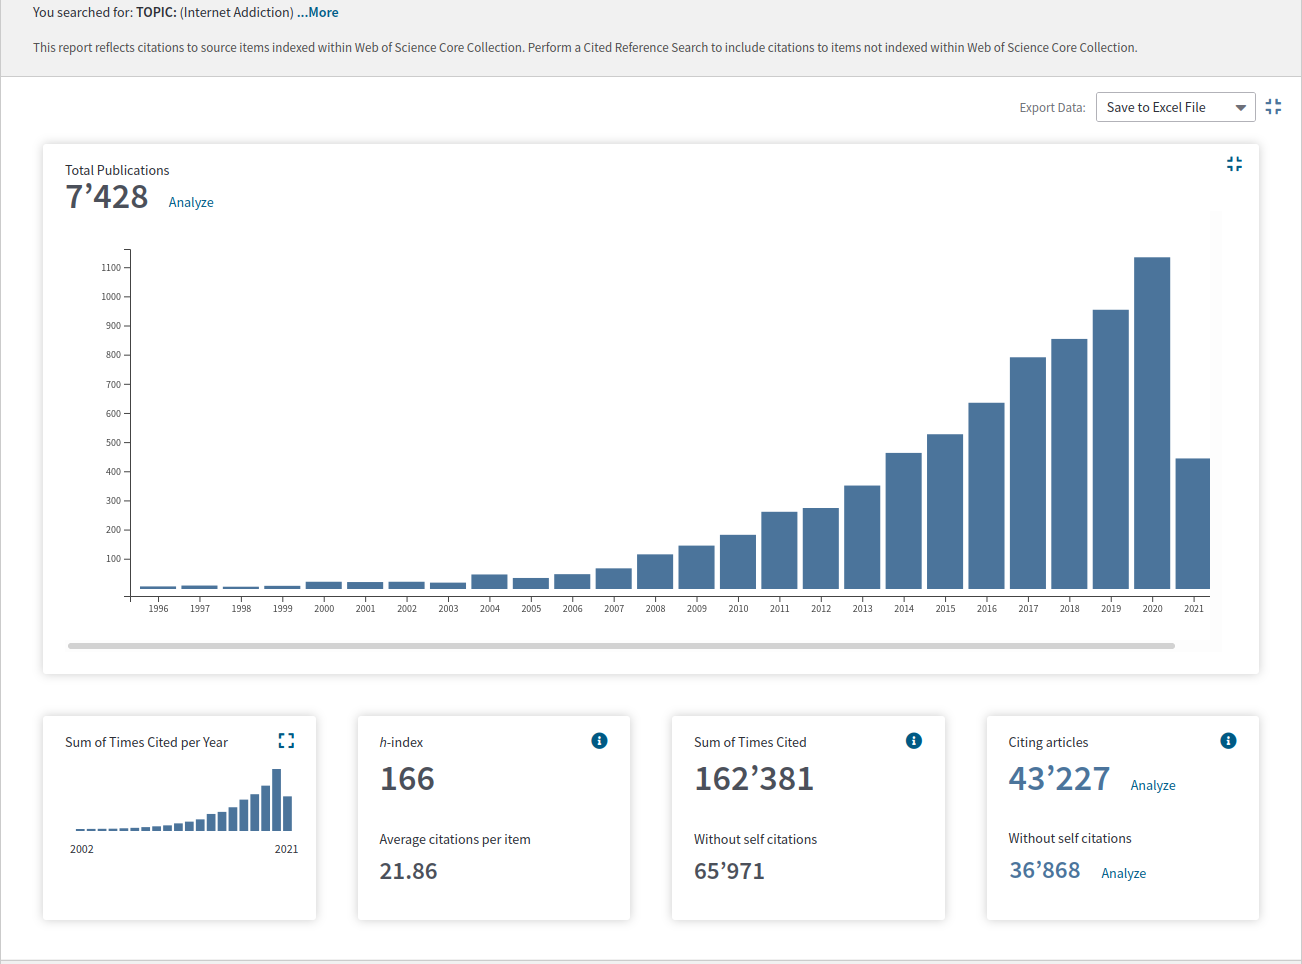
\includegraphics[width = \textwidth]{figures/Internet_addiction.png}
        \caption{The screen-shot of a \href{https://apps.webofknowledge.com/}{Web of Science} citation report created on July 7th, 2021, for the search term \textquote{Internet Addiction}.}
        \label{fig:internet_addiction}
    \end{subfigure}
    \begin{subfigure}[b]{0.83\textwidth}
        \centering
    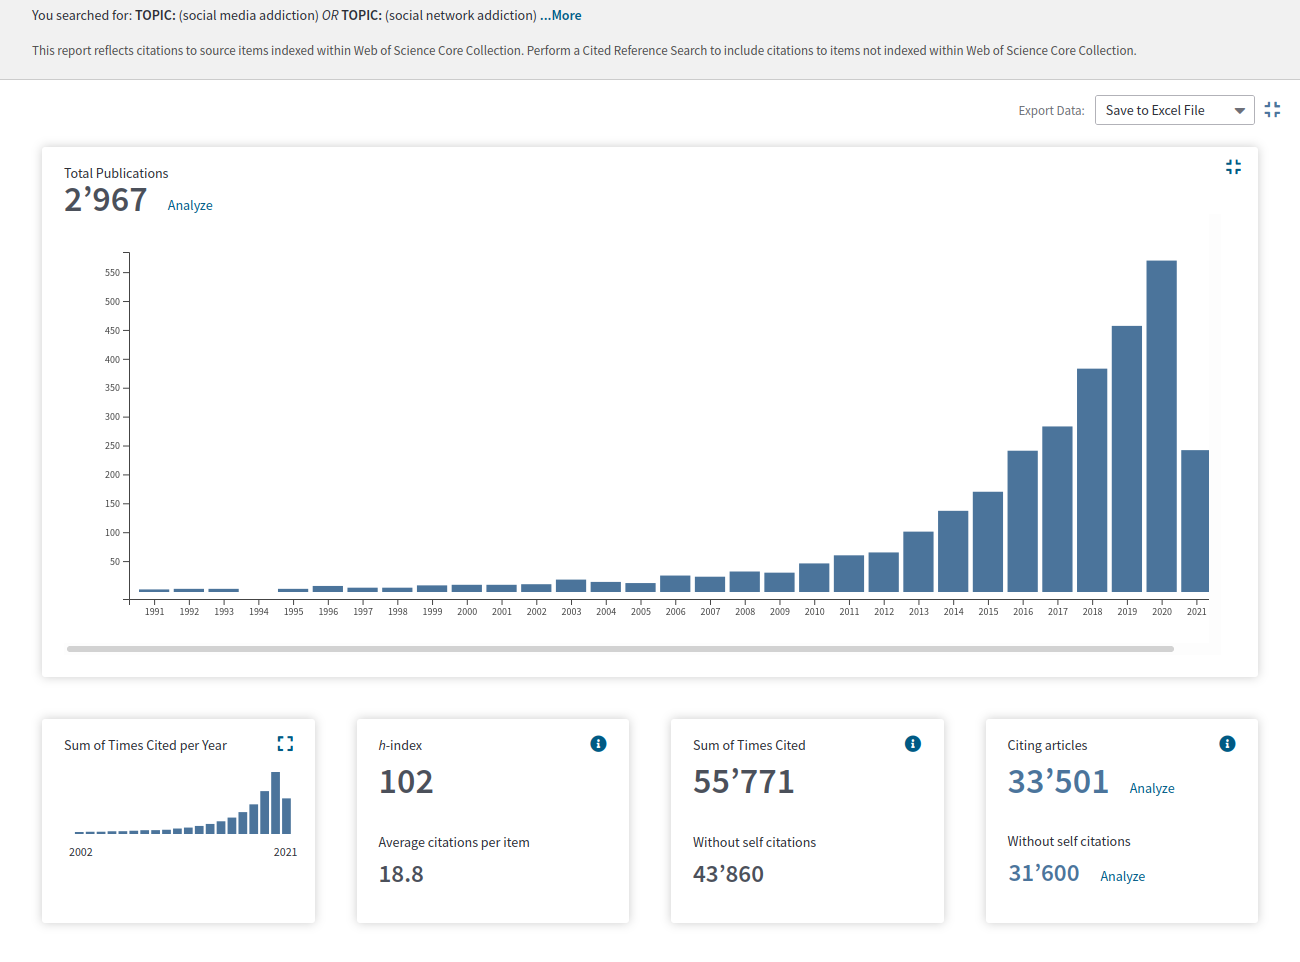
\includegraphics[width = \textwidth]{figures/Social_media_addiction.png}
    \caption{The screen-shot of a \href{https://apps.webofknowledge.com/}{Web of Science} citation report created on July 7th, 2021, for \textquote{TOPIC:(Social Media Addiction) OR TOPCI:(Social Network Addiction)}.}
    \label{fig:sns_addiction}
    \end{subfigure}
\end{figure}

\begin{figure}
    \centering
    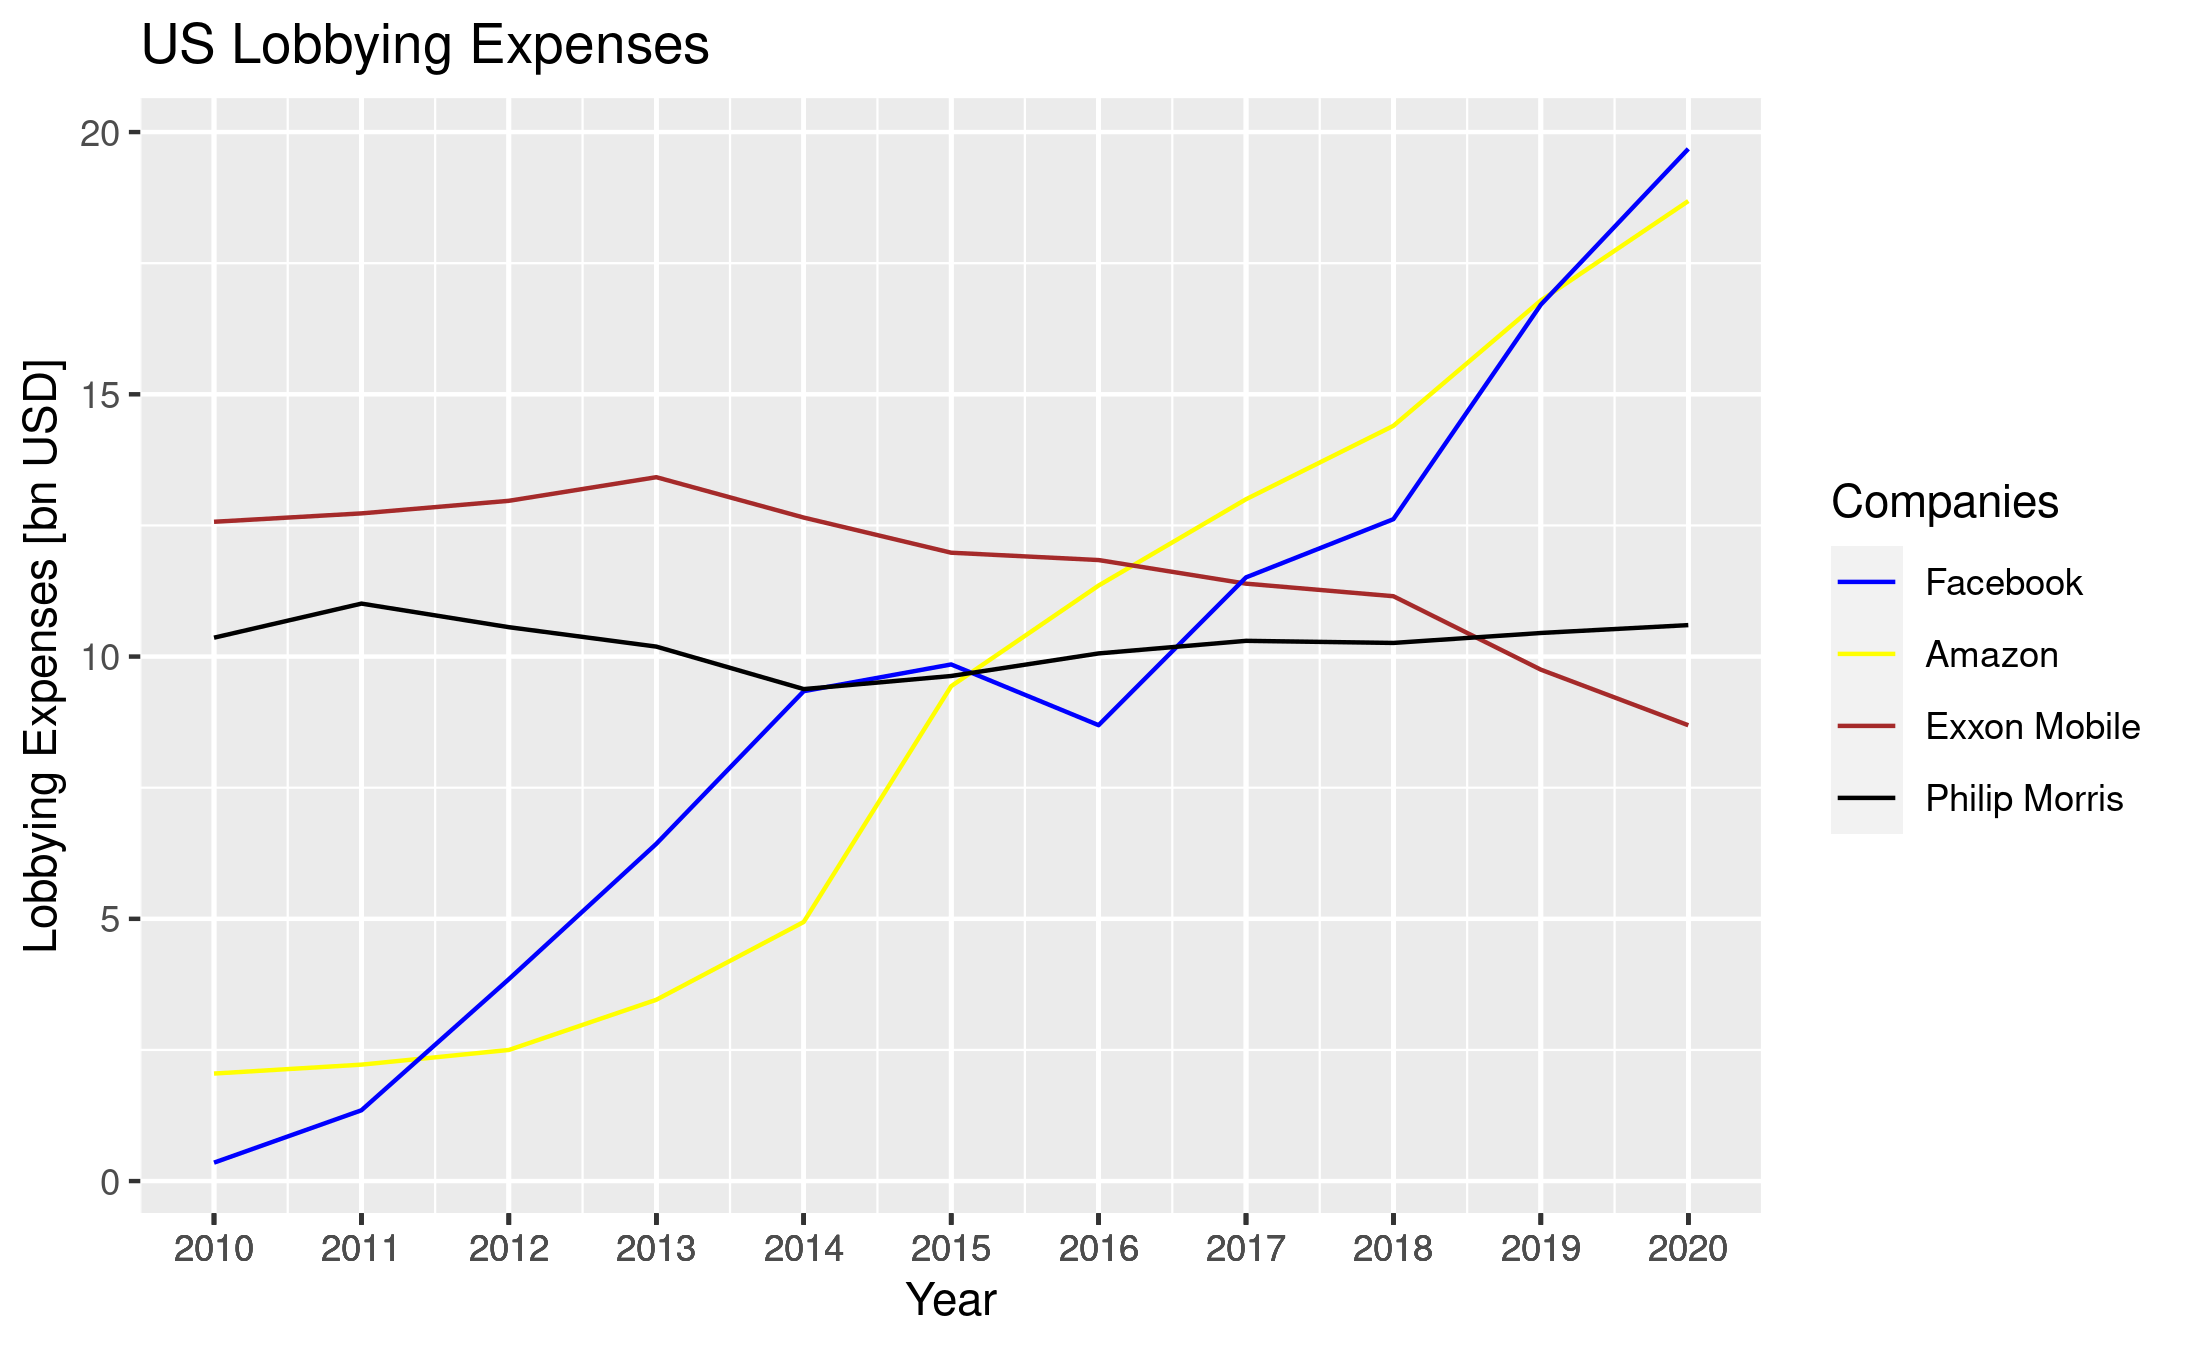
\includegraphics[width=\textwidth]{figures/Lobbying_Expenditures.png}
    \caption{Lobbying Expenditures of: Facebook, Amazon, Exxon Mobile, and Philip Morris over Time, reproduced from \citep{chung_big_2021} with data from \textit{The Center for Responsive Politics} (\href{https://www.opensecrets.org/}{www.opensecrets.org}).}
    \label{fig:lob_exp}
\end{figure}
\section{References}
\sloppy
%\printbibliography[heading=none]

\end{document}

%\begin{multicols}{4}
%\multido{\i=0+1}{"10000}{% from U+0000 to U+FFFF
%  \iffontchar\font\i
%    \makebox[3em][l]{\i}%
%    \XeTeXglyph\i\endgraf
%  \fi
%}
%\end{multicols}